\section{Результаты измерений}
\begin{figure}[ht!]
    \center{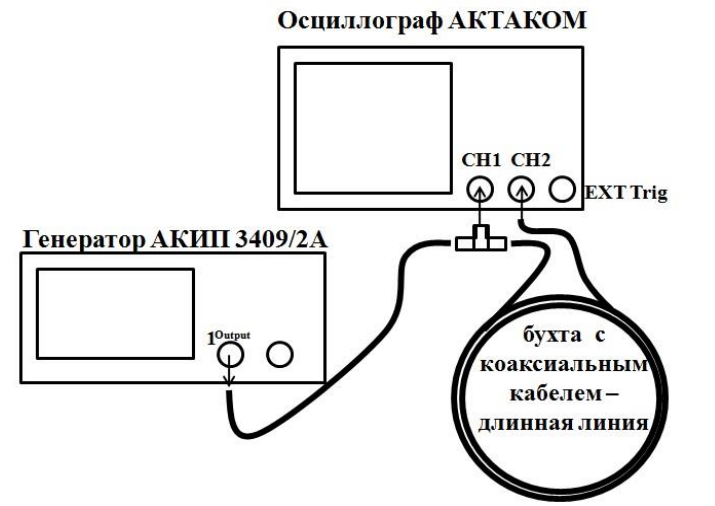
\includegraphics[width=0.8\linewidth]{../img/fig2.png}}
\end{figure}
\begin{figure}[ht!]
    \center{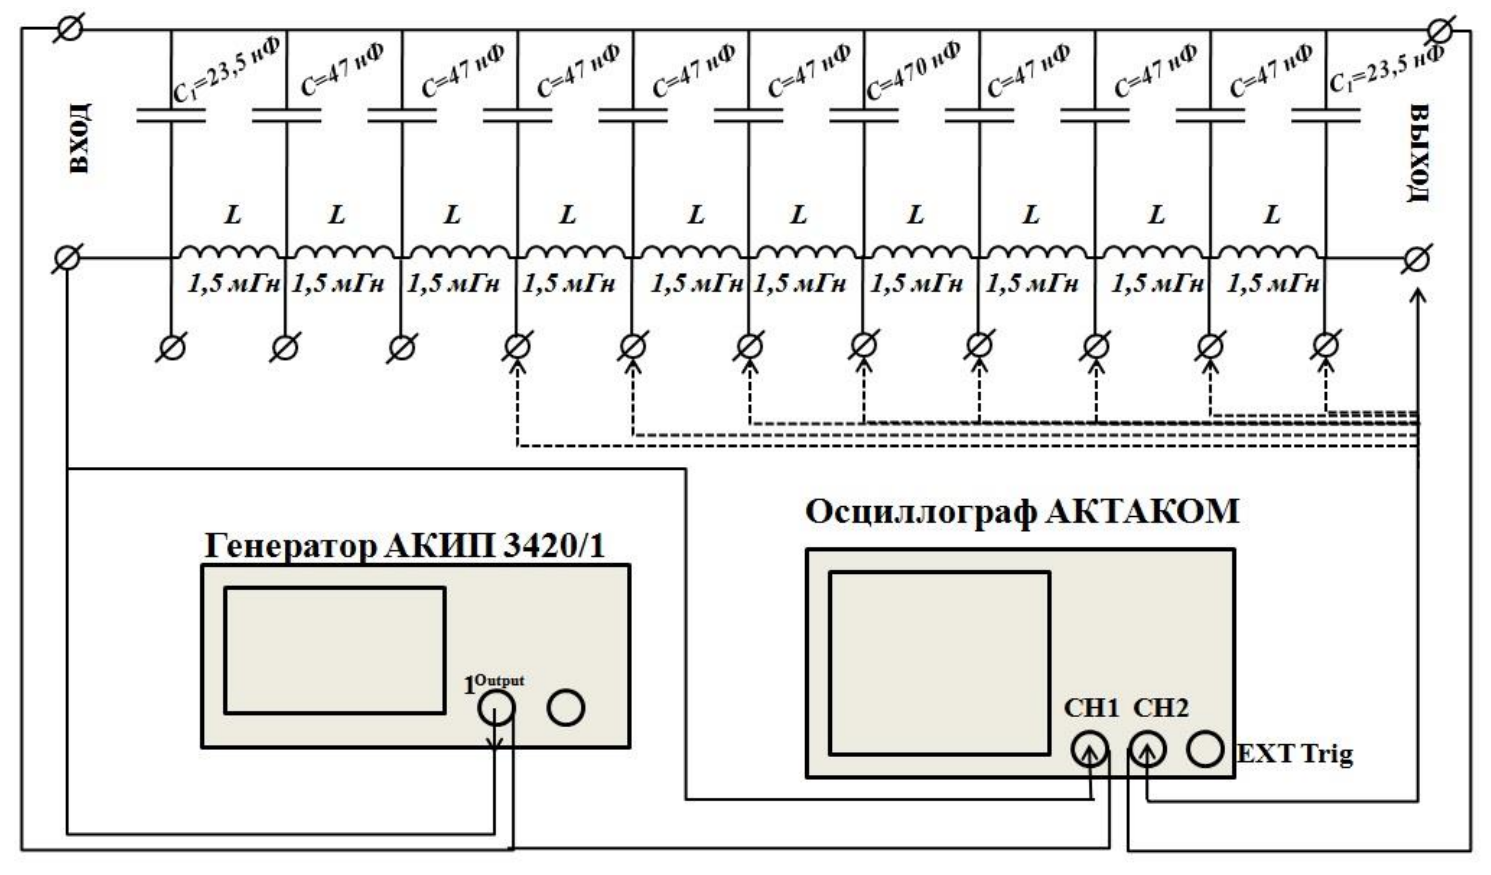
\includegraphics[width=0.8\linewidth]{../img/fig3.png}}
\end{figure}

\begin{table}[!ht]
    \centering
    \caption{Резонансные частоты}
    \begin{tabular}{|l|l|l|l|}
\hline
$\text{синус согл.},\;\text{МГц}$ & $\text{синус. без нагр.},\;\text{МГц}$ & $\text{прям. согл.},\;\text{МГц}$ & $\text{прям. без нагр.},\;\text{МГц}$\\\hline
$19{,}933$ & $20{,}0$ & $20{,}0$ & $20{,}0$\\\hline
$15{,}933$ & $16{,}0$ & $16{,}0$ & $16{,}0$\\\hline
$11{,}943$ & $12{,}0$ & $12{,}0$ & $12{,}0$\\\hline
$7{,}94$ & $8{,}0$ & $8{,}0$ & $8{,}0$\\\hline
$3{,}945$ & $4{,}0$ & $4{,}0$ & $4{,}0$\\\hline
\end{tabular}

\end{table}

Фазовая скорость
\[
    V_{\text{ф}} = 2\cdot 10^{8}\;\text{м} / \text{с}
\]
Дисперсия почти отсутствует.

\begin{table}[!ht]
    \centering
    \caption{АЧХ}
    \begin{tabular}{|l|l|}
\hline
$f,\;\text{МГц}$ & $V,\;\text{В}$\\\hline
$1{,}0$ & $25{,}2$\\\hline
$2{,}0$ & $25{,}0$\\\hline
$3{,}0$ & $24{,}4$\\\hline
$4{,}0$ & $24{,}2$\\\hline
$5{,}0$ & $23{,}8$\\\hline
$6{,}0$ & $23{,}4$\\\hline
$7{,}0$ & $23{,}0$\\\hline
$8{,}0$ & $22{,}8$\\\hline
$9{,}0$ & $22{,}6$\\\hline
$10{,}0$ & $22{,}6$\\\hline
$11{,}0$ & $22{,}2$\\\hline
$12{,}0$ & $22{,}1$\\\hline
$13{,}0$ & $21{,}8$\\\hline
$14{,}0$ & $21{,}8$\\\hline
$15{,}0$ & $21{,}4$\\\hline
$16{,}0$ & $21{,}4$\\\hline
$17{,}0$ & $21{,}2$\\\hline
$18{,}0$ & $21{,}2$\\\hline
$19{,}0$ & $21{,}0$\\\hline
$20{,}0$ & $21{,}0$\\\hline
$21{,}0$ & $20{,}6$\\\hline
$22{,}0$ & $20{,}6$\\\hline
$23{,}0$ & $20{,}2$\\\hline
$24{,}0$ & $20{,}3$\\\hline
$25{,}0$ & $19{,}8$\\\hline
$26{,}0$ & $20{,}0$\\\hline
$27{,}0$ & $19{,}4$\\\hline
$28{,}0$ & $19{,}7$\\\hline
$29{,}0$ & $19{,}2$\\\hline
$30{,}0$ & $19{,}2$\\\hline
$31{,}0$ & $19{,}0$\\\hline
$32{,}0$ & $19{,}0$\\\hline
$33{,}0$ & $18{,}6$\\\hline
$34{,}0$ & $18{,}6$\\\hline
$35{,}0$ & $18{,}4$\\\hline
$36{,}0$ & $18{,}2$\\\hline
$37{,}0$ & $17{,}8$\\\hline
$38{,}0$ & $17{,}9$\\\hline
$39{,}0$ & $17{,}7$\\\hline
$40{,}0$ & $17{,}4$\\\hline
\end{tabular}

\end{table}

\begin{table}[!ht]
    \centering
    \caption{ФЧХ}
    \begin{tabular}{|l|l|}
\hline
$f,\;\text{МГц}$ & $\phi$\\\hline
$4{,}0$ & $0{,}09948376736367678$\\\hline
$4{,}2$ & $0{,}4014257279586958$\\\hline
$4{,}4$ & $0{,}7330382858376184$\\\hline
$4{,}6$ & $1{,}0471975511965976$\\\hline
$4{,}8$ & $1{,}3508848410436112$\\\hline
$5{,}0$ & $1{,}6650441064025905$\\\hline
$5{,}2$ & $1{,}99142067652553$\\\hline
$5{,}4$ & $2{,}2689280275926285$\\\hline
$5{,}6$ & $2{,}6179938779914944$\\\hline
$5{,}8$ & $2{,}91469985083053$\\\hline
$6{,}0$ & $3{,}036872898470133$\\\hline
$6{,}2$ & $2{,}6878070480712677$\\\hline
$6{,}4$ & $2{,}356194490192345$\\\hline
$6{,}6$ & $2{,}059488517353309$\\\hline
$6{,}8$ & $1{,}7627825445142729$\\\hline
$7{,}0$ & $1{,}4486232791552935$\\\hline
$7{,}2$ & $1{,}117010721276371$\\\hline
$7{,}4$ & $0{,}8377580409572782$\\\hline
$7{,}6$ & $0{,}49741883681838395$\\\hline
$7{,}8$ & $0{,}19722220547535926$\\\hline
$8{,}0$ & $0{,}12217304763960307$\\\hline
$8{,}2$ & $0{,}4537856055185257$\\\hline
$8{,}4$ & $0{,}7504915783575618$\\\hline
$8{,}6$ & $1{,}0821041362364843$\\\hline
$8{,}8$ & $1{,}3788101090755203$\\\hline
$9{,}0$ & $1{,}6929693744344996$\\\hline
\end{tabular}

\end{table}

\begin{figure}[ht!]
    \center{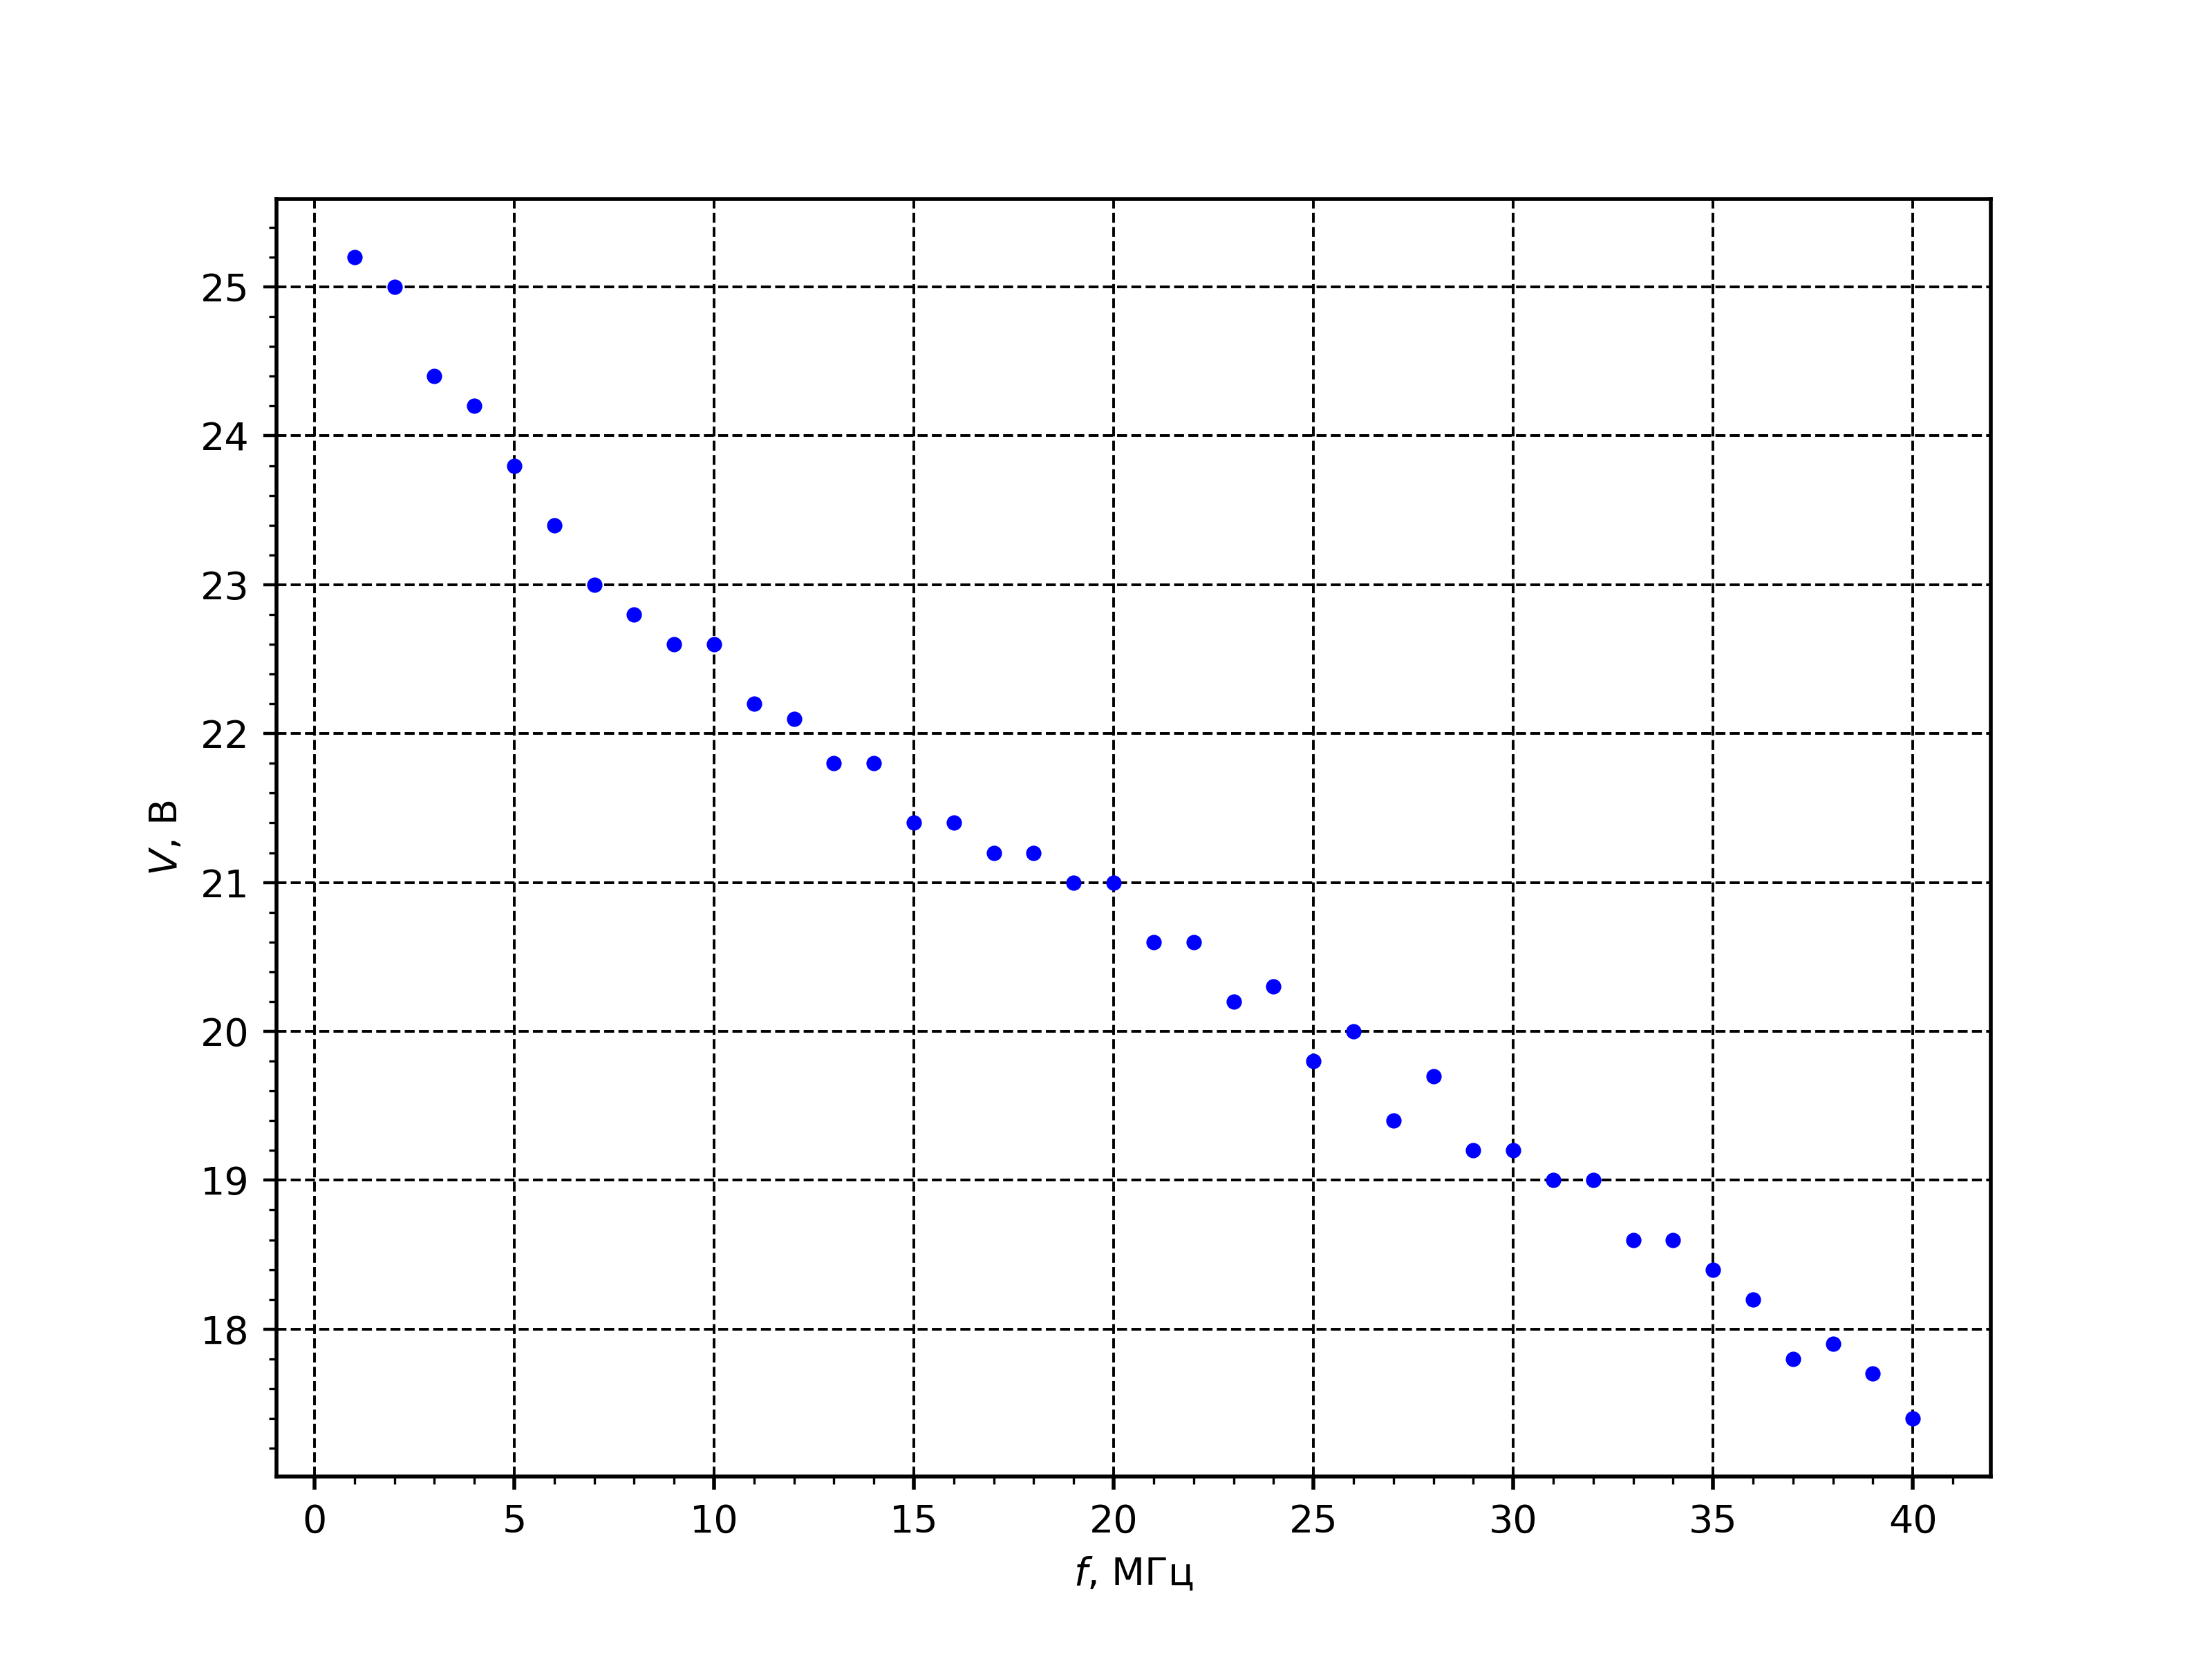
\includegraphics[width=0.8\linewidth]{../img/achh.png}}
\end{figure}
\begin{figure}[ht!]
    \center{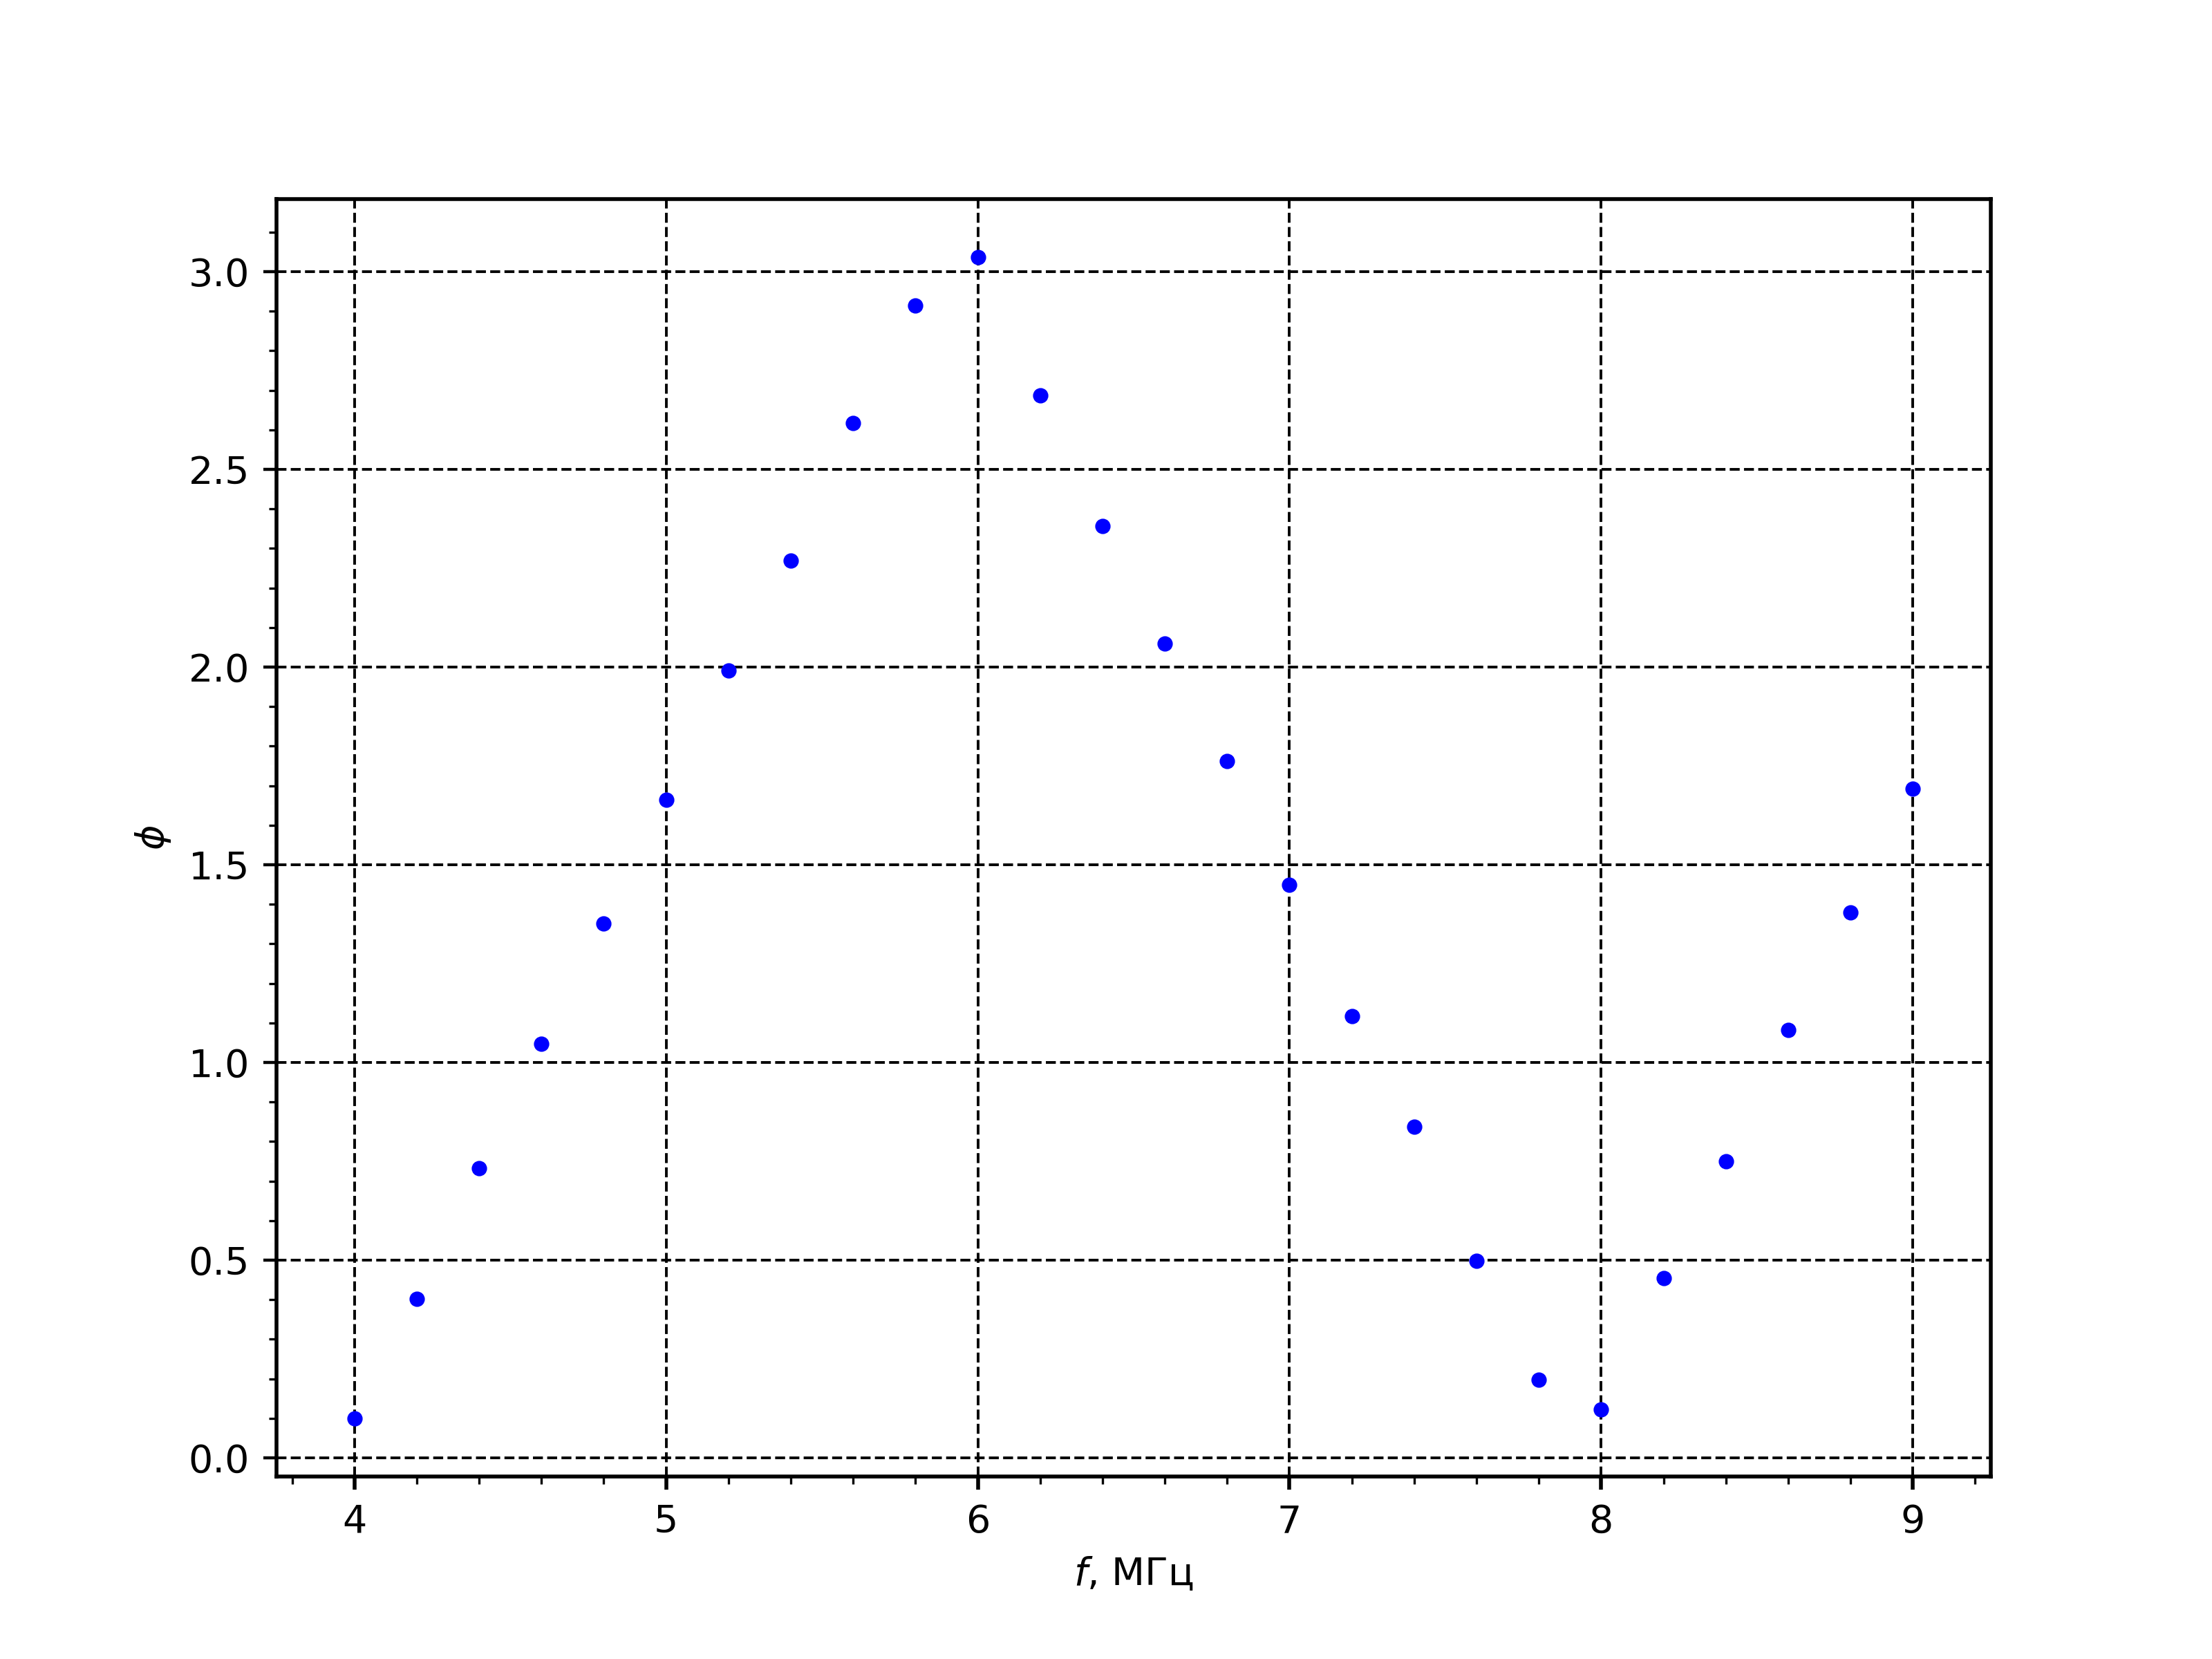
\includegraphics[width=0.8\linewidth]{../img/fchh.png}}
\end{figure}


Для описания характеричтик коаксиального кабеля уравнения удобно переписать следующим образом:
\[
    y_{1} = \frac{L_{x}C_{x}}{c^{2}}x^{1}
\]
\[
    x_{1}=w^{2}
\]
\[
    y_{1}=k(w)^{2}- \alpha (w)^{2}
\]

По наклону прямой можно определить $L_{x}C_{x}$, а зная волновое сопротивление кабеля,
определить $L_{x}$ и $C_{x}$.

\begin{figure}[ht!]
    \center{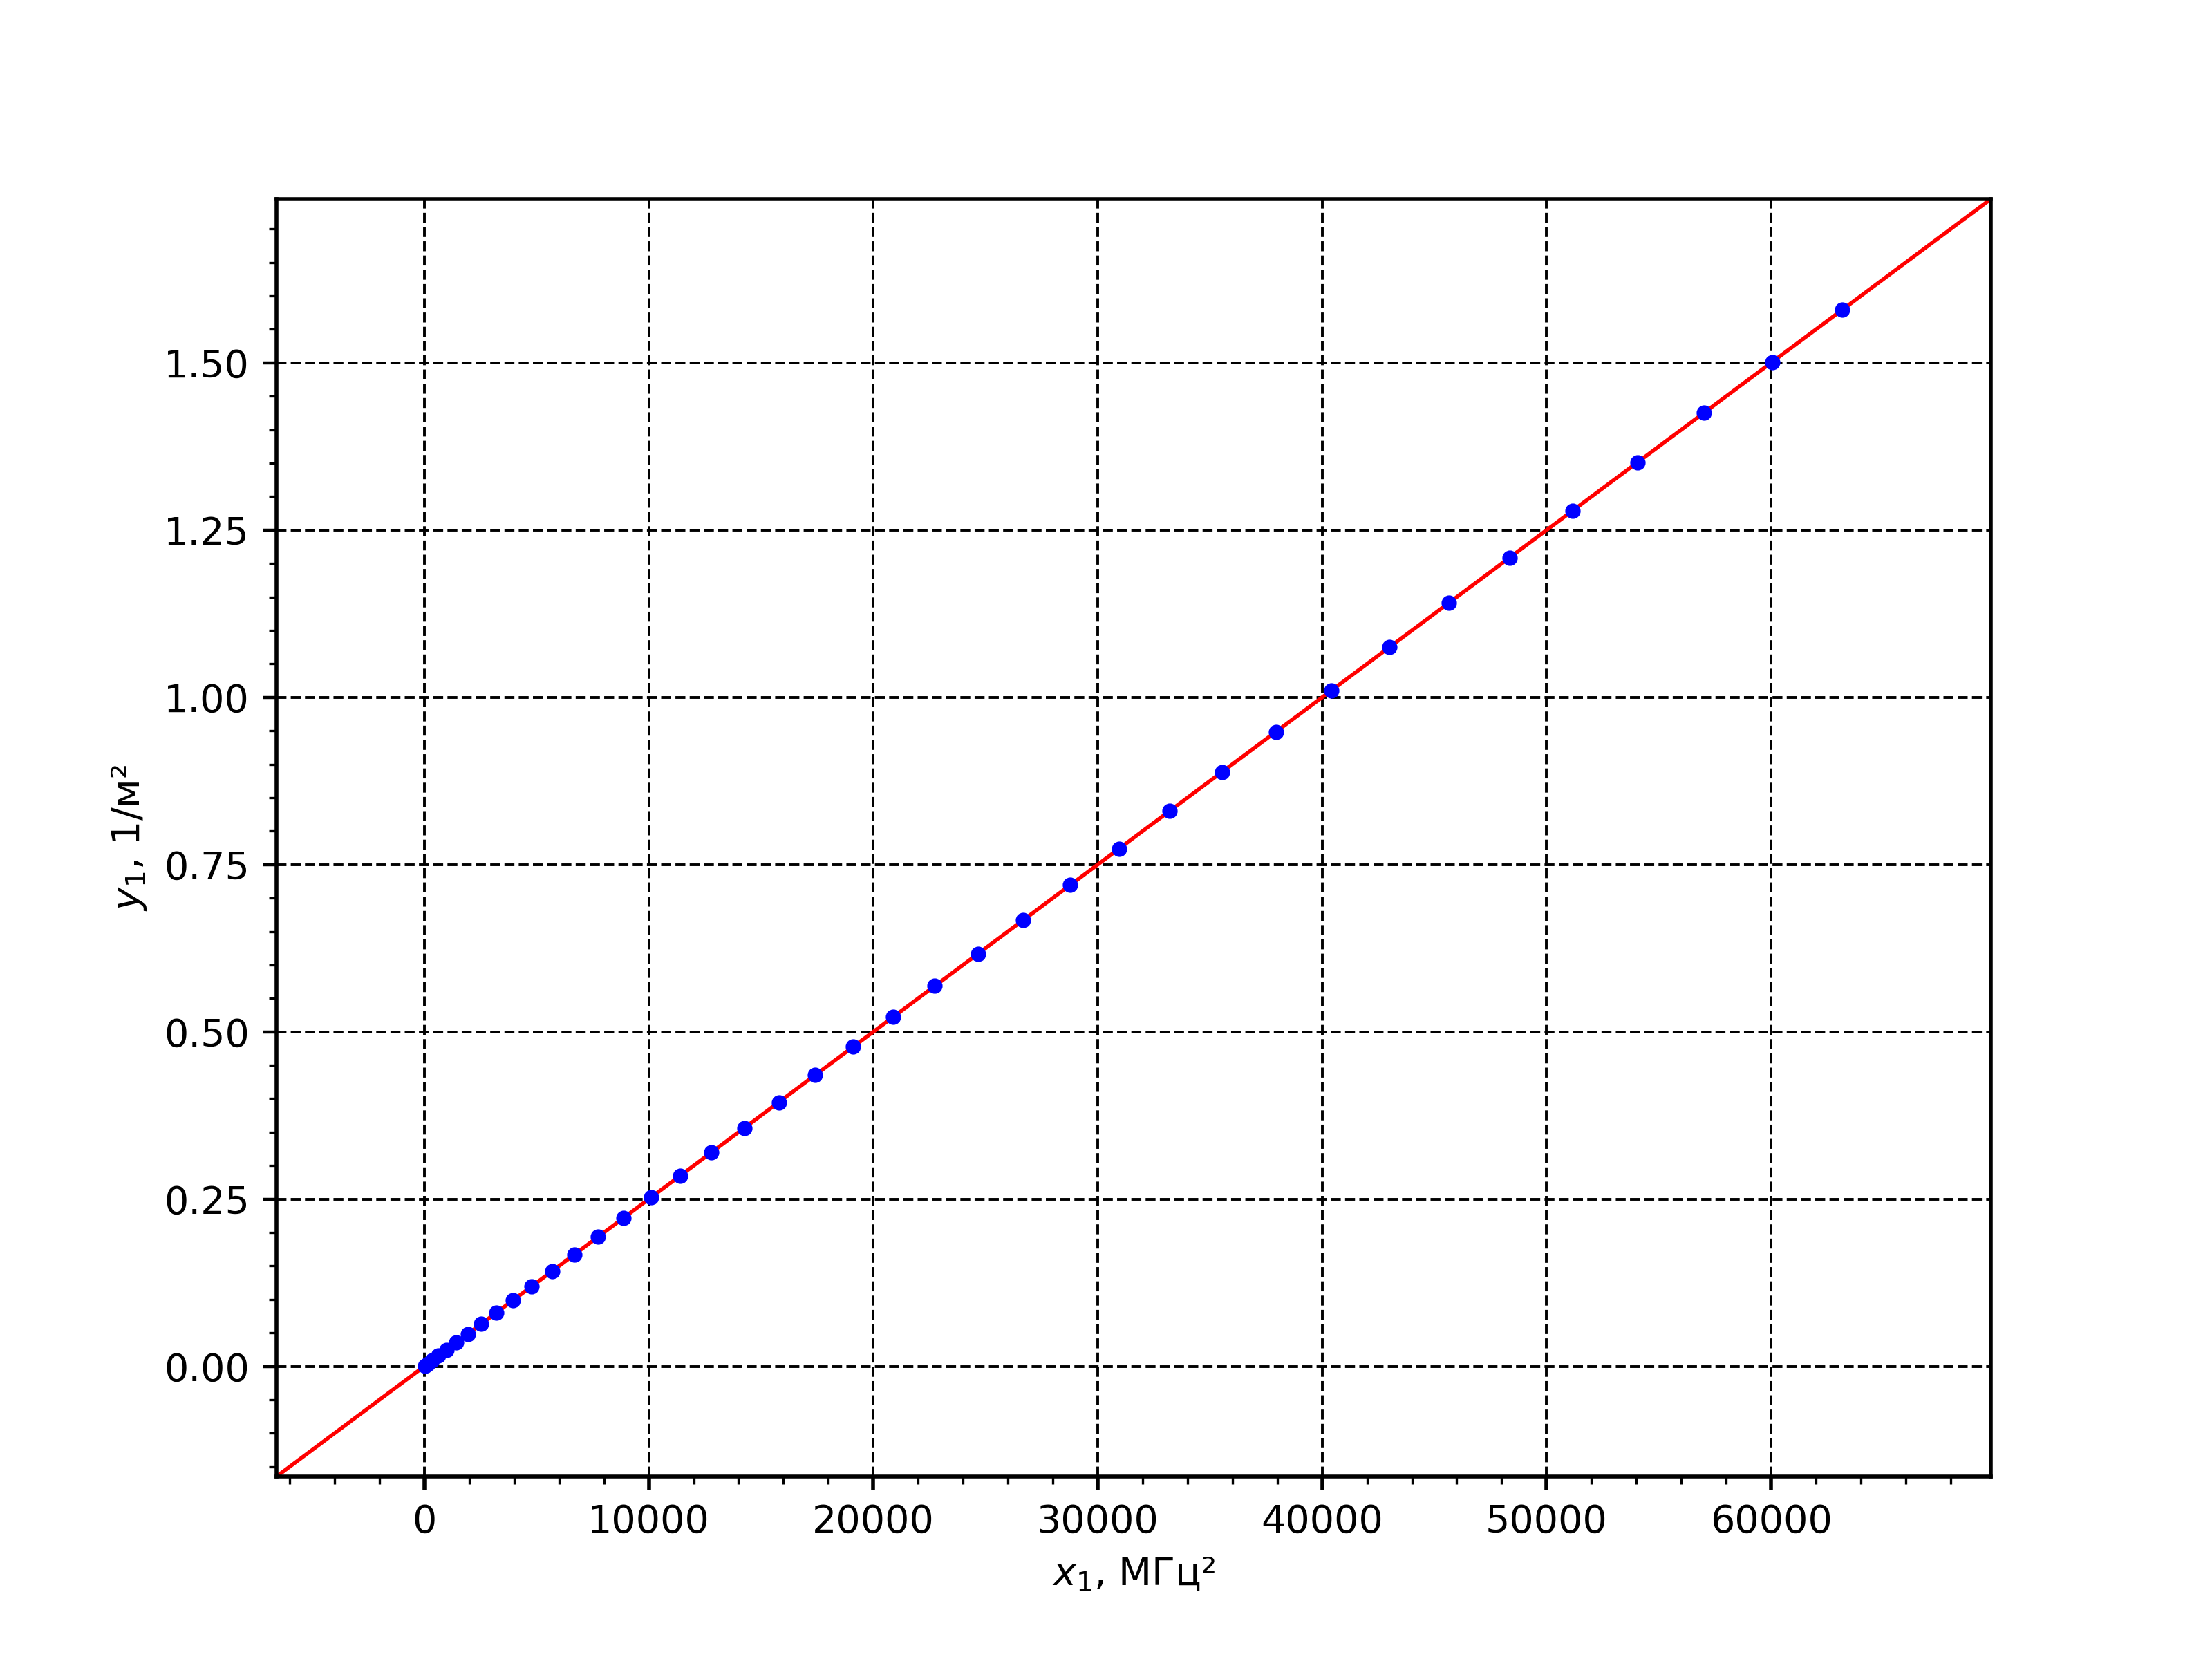
\includegraphics[width=0.8\linewidth]{../img/line1.png}}
\end{figure}
\[
    k_{1} = \left(2499894 \pm 2\right)\cdot 10^{-11}\;\text{МГц}^{-2}\cdot\text{м}^{-2}
\]
\[
    L_{x} \approx 2{,}75\;\text{мкГн}/\text{м}
\]
\[
    C_{x} \approx 0{,}1\;\text{нФ}/\text{м}
\]


Из этих величин и геометрических параметров можно найти $ \varepsilon$ и $ \mu$.

\[
    \mu \approx 1{,}18
\]
\[
    \varepsilon \approx 1{,}9
\]


Удельную проводимость $ \sigma$ материала проводников можно определить двумя методами.

\textbf{Метод А}

\[
    \alpha(w) = \frac{1}{l}\ln\left(\frac{U_{0}}{U_{\text{н}}}\right) = R_{x}C_{x}\frac{V_{\text{ф}}}{2}    
\]
Если взять удельную проводимость для меди и подставить в известное выражение для характерной толщины скин-слоя:
\[
    \delta = \frac{c}{2 \pi \sqrt{\nu\sigma}}
\]
то окажется, что даже при минимальной частоте $\nu=1\;\text{МГц}$  эта толщина будет равна около
$65\;\text{мкм}$, что примерно в десять раз меньше радиуса центрального проводника.
 При больших частотах характерная толщина скин-слоя ещё меньше. Поэтому для упрощения будем предполагать, что весь ток сосредоточен в приповерхностном слое и потери, связанные с джоулевым нагревом описываются следующим выражением:
 \[
     dN=\frac{(dU)^{2}}{dR}
 \]
 \[
     dR=\frac{dx}{\sigma \pi d}\frac{2}{ \delta}
 \]
 Погонное сопротивление с учётом скин-эффекта можно определить следующим образом:
 \[
     R_{x} = \frac{2}{\sigma \pi d \delta} = \frac{4\sqrt{\nu}}{\sqrt{\sigma}cd}    
 \]
\[
    \alpha(w) = \frac{4}{\sqrt{\sigma}d}C_{x}\frac{V_{\text{ф}}}{c}\sqrt{\nu}
\]

\[
    y_{2} = \frac{4}{\sqrt{\sigma}d}C_{x}\frac{V_{\text{ф}}}{c}x_{2}
\]
\[
    x_{2} = \sqrt{\nu}
\]
\[
    y_{2} = \alpha(w)
\]

По наклону прямой можно определить $\sigma$
\[
    \sigma = \left(\frac{2C_{x}V_{\text{ф}}}{cd\left(\Delta y_{2}/ \Delta x_{2}\right)}\right)^{2}
\]

\begin{figure}[ht!]
    \center{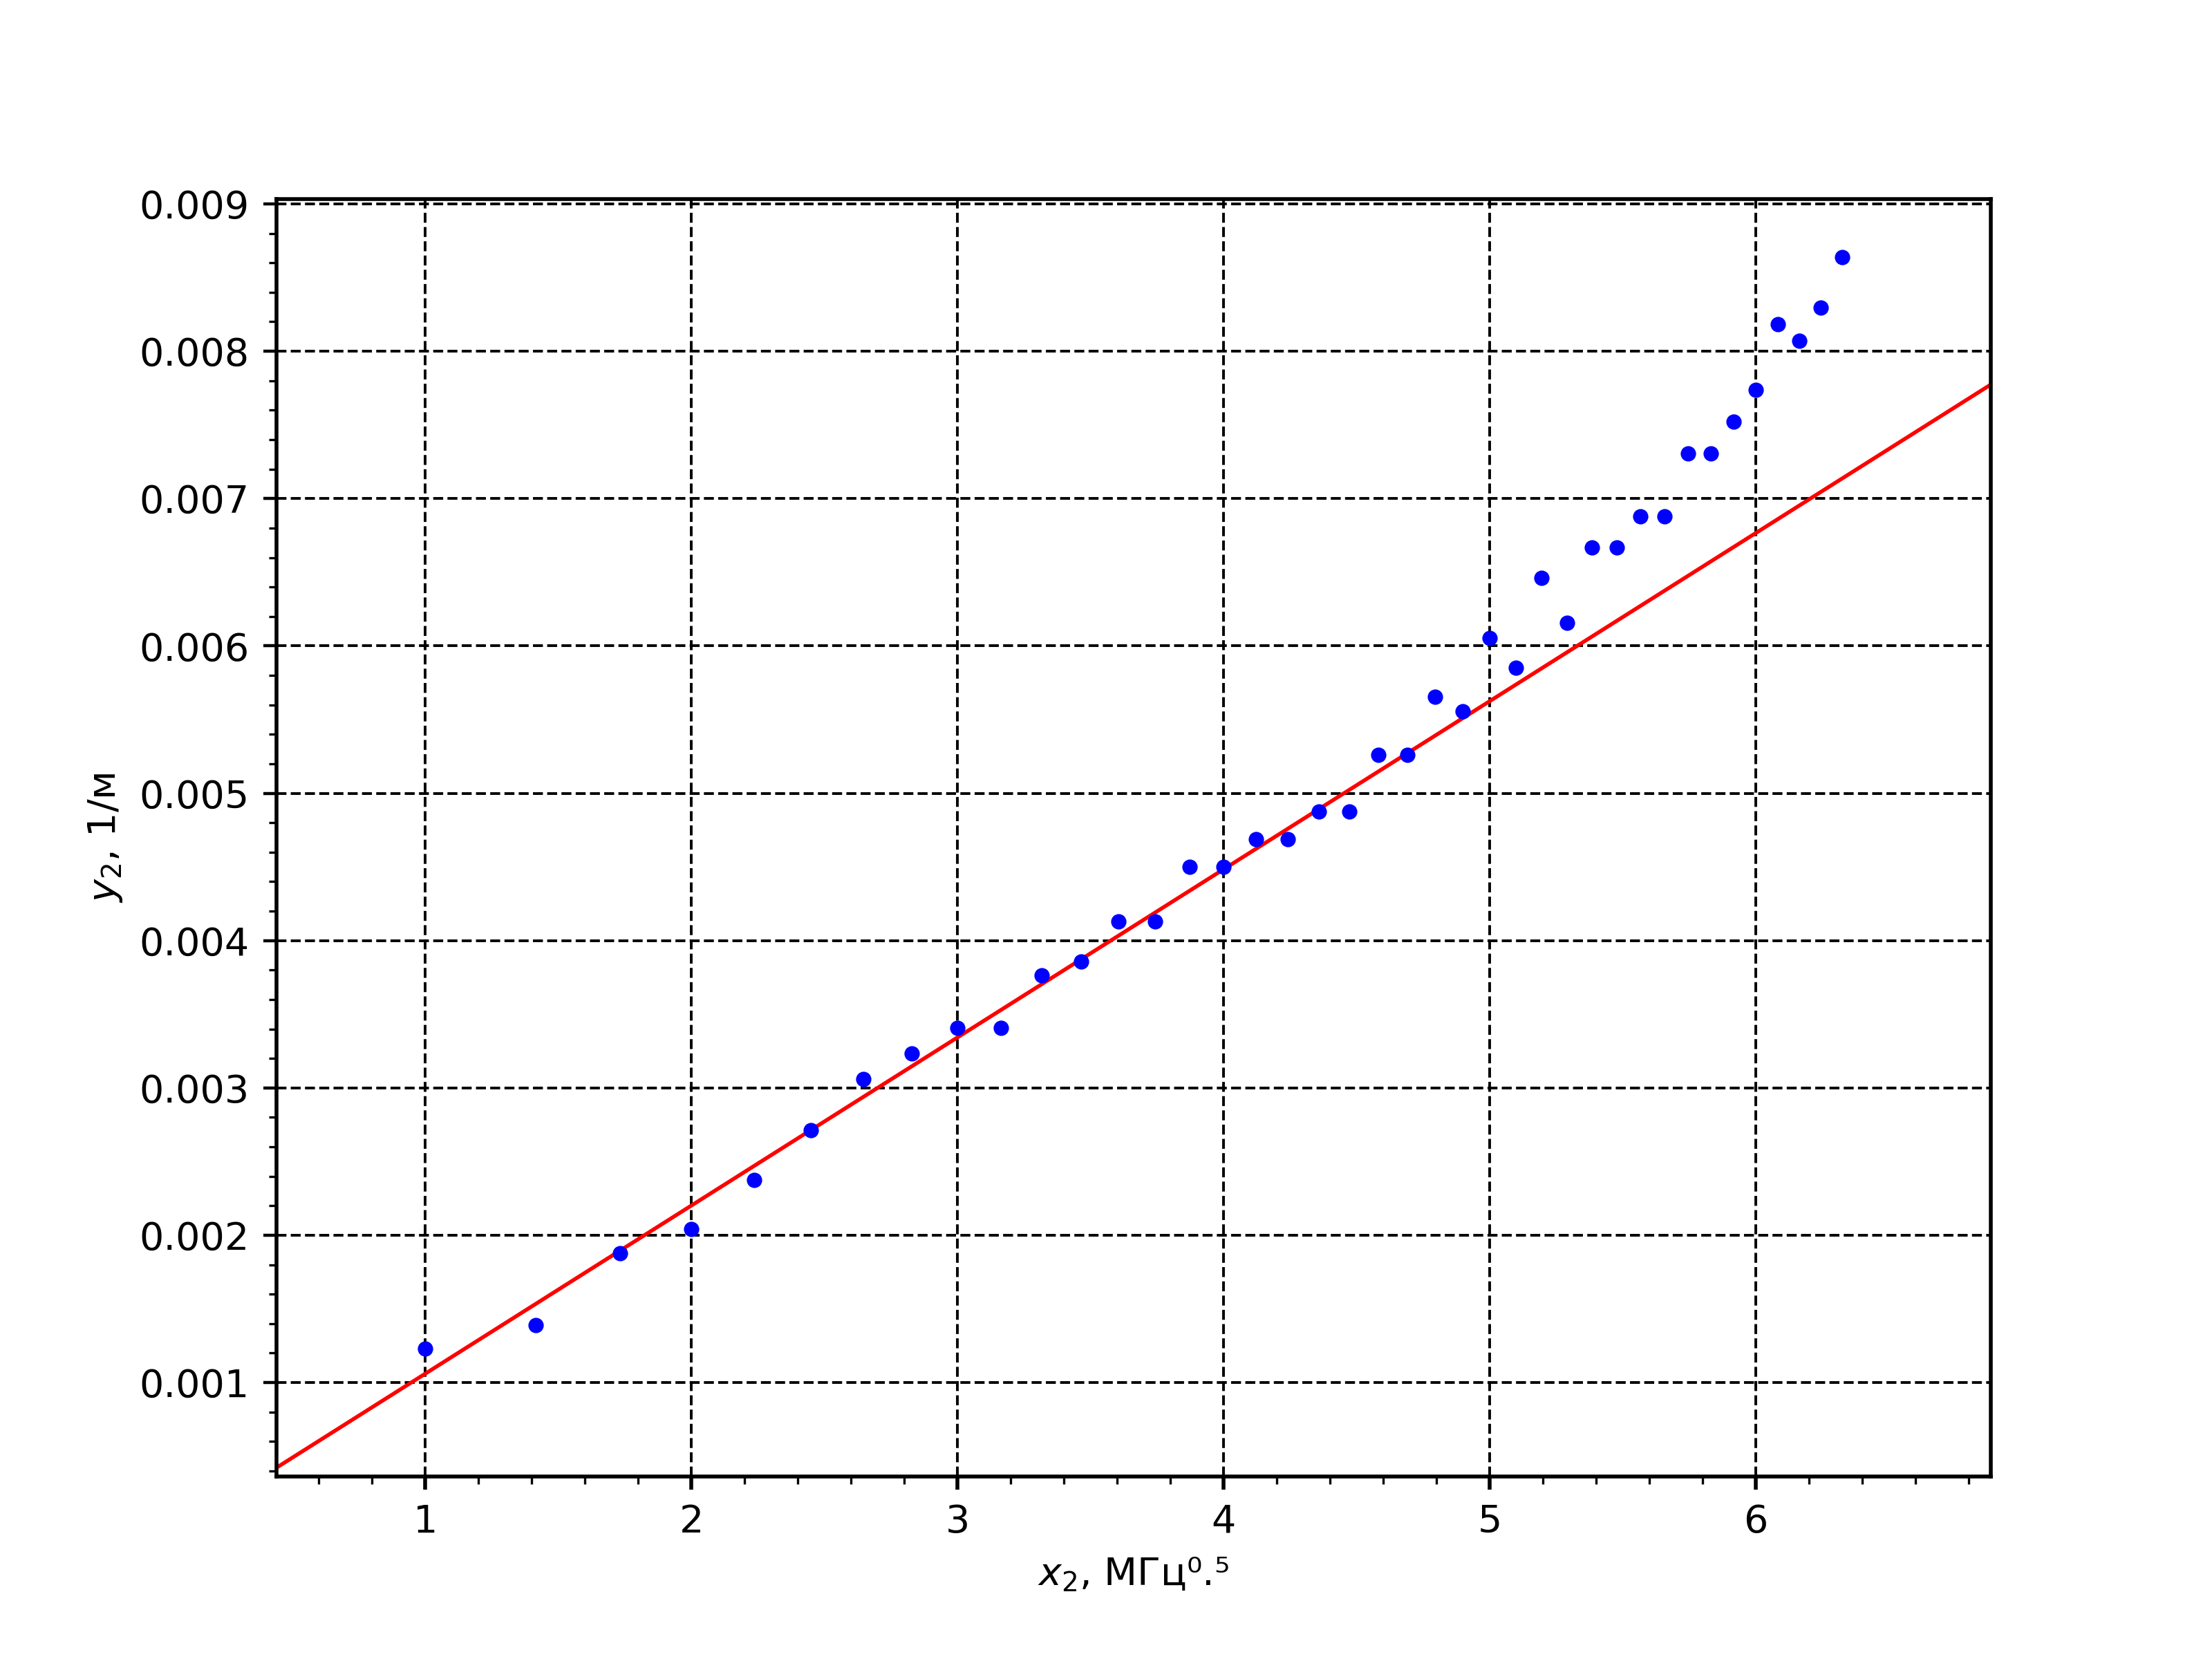
\includegraphics[width=0.8\linewidth]{../img/line2.png}}
\end{figure}
\[
    k_{2} = \left(114 \pm 2\right)\cdot 10^{-5}\;\text{МГц}^{-0.5}\cdot\text{м}^{-1.0}
\]
\[
    \sigma = \left(66 \pm 3\right)\cdot 10^{6}\;\text{См} / \text{м}
\]


\textbf{Метод Б}
\[
    2 \alpha k = wR_{x}C_{x}
\]
Зная амплитуду колебаний и сдвиг фазы в конце длинной линии относительно входного
сигнала экспериментально можно определить как $ \alpha(w)$ так и $k(w)$
\[
    y_{3} = \frac{4 \pi C_{x}}{\sqrt{\sigma}dc}x_{3}
\]
\[
    x_{3} = \nu^{3/2}
\]
\[
    y_{3} = \alpha(w)k(w) = \frac{1}{l}\ln\left(\frac{U_{0}}{U_{\text{н}}}\right)\frac{ \Delta \varphi}{l}
\]
По наклону прямой
\[
    \sigma = \left(\frac{4 \pi C_{x}}{dc\left(\Delta y_{3}/ \Delta x_{3}\right)}\right)^{2}
\]

\begin{figure}[ht!]
    \center{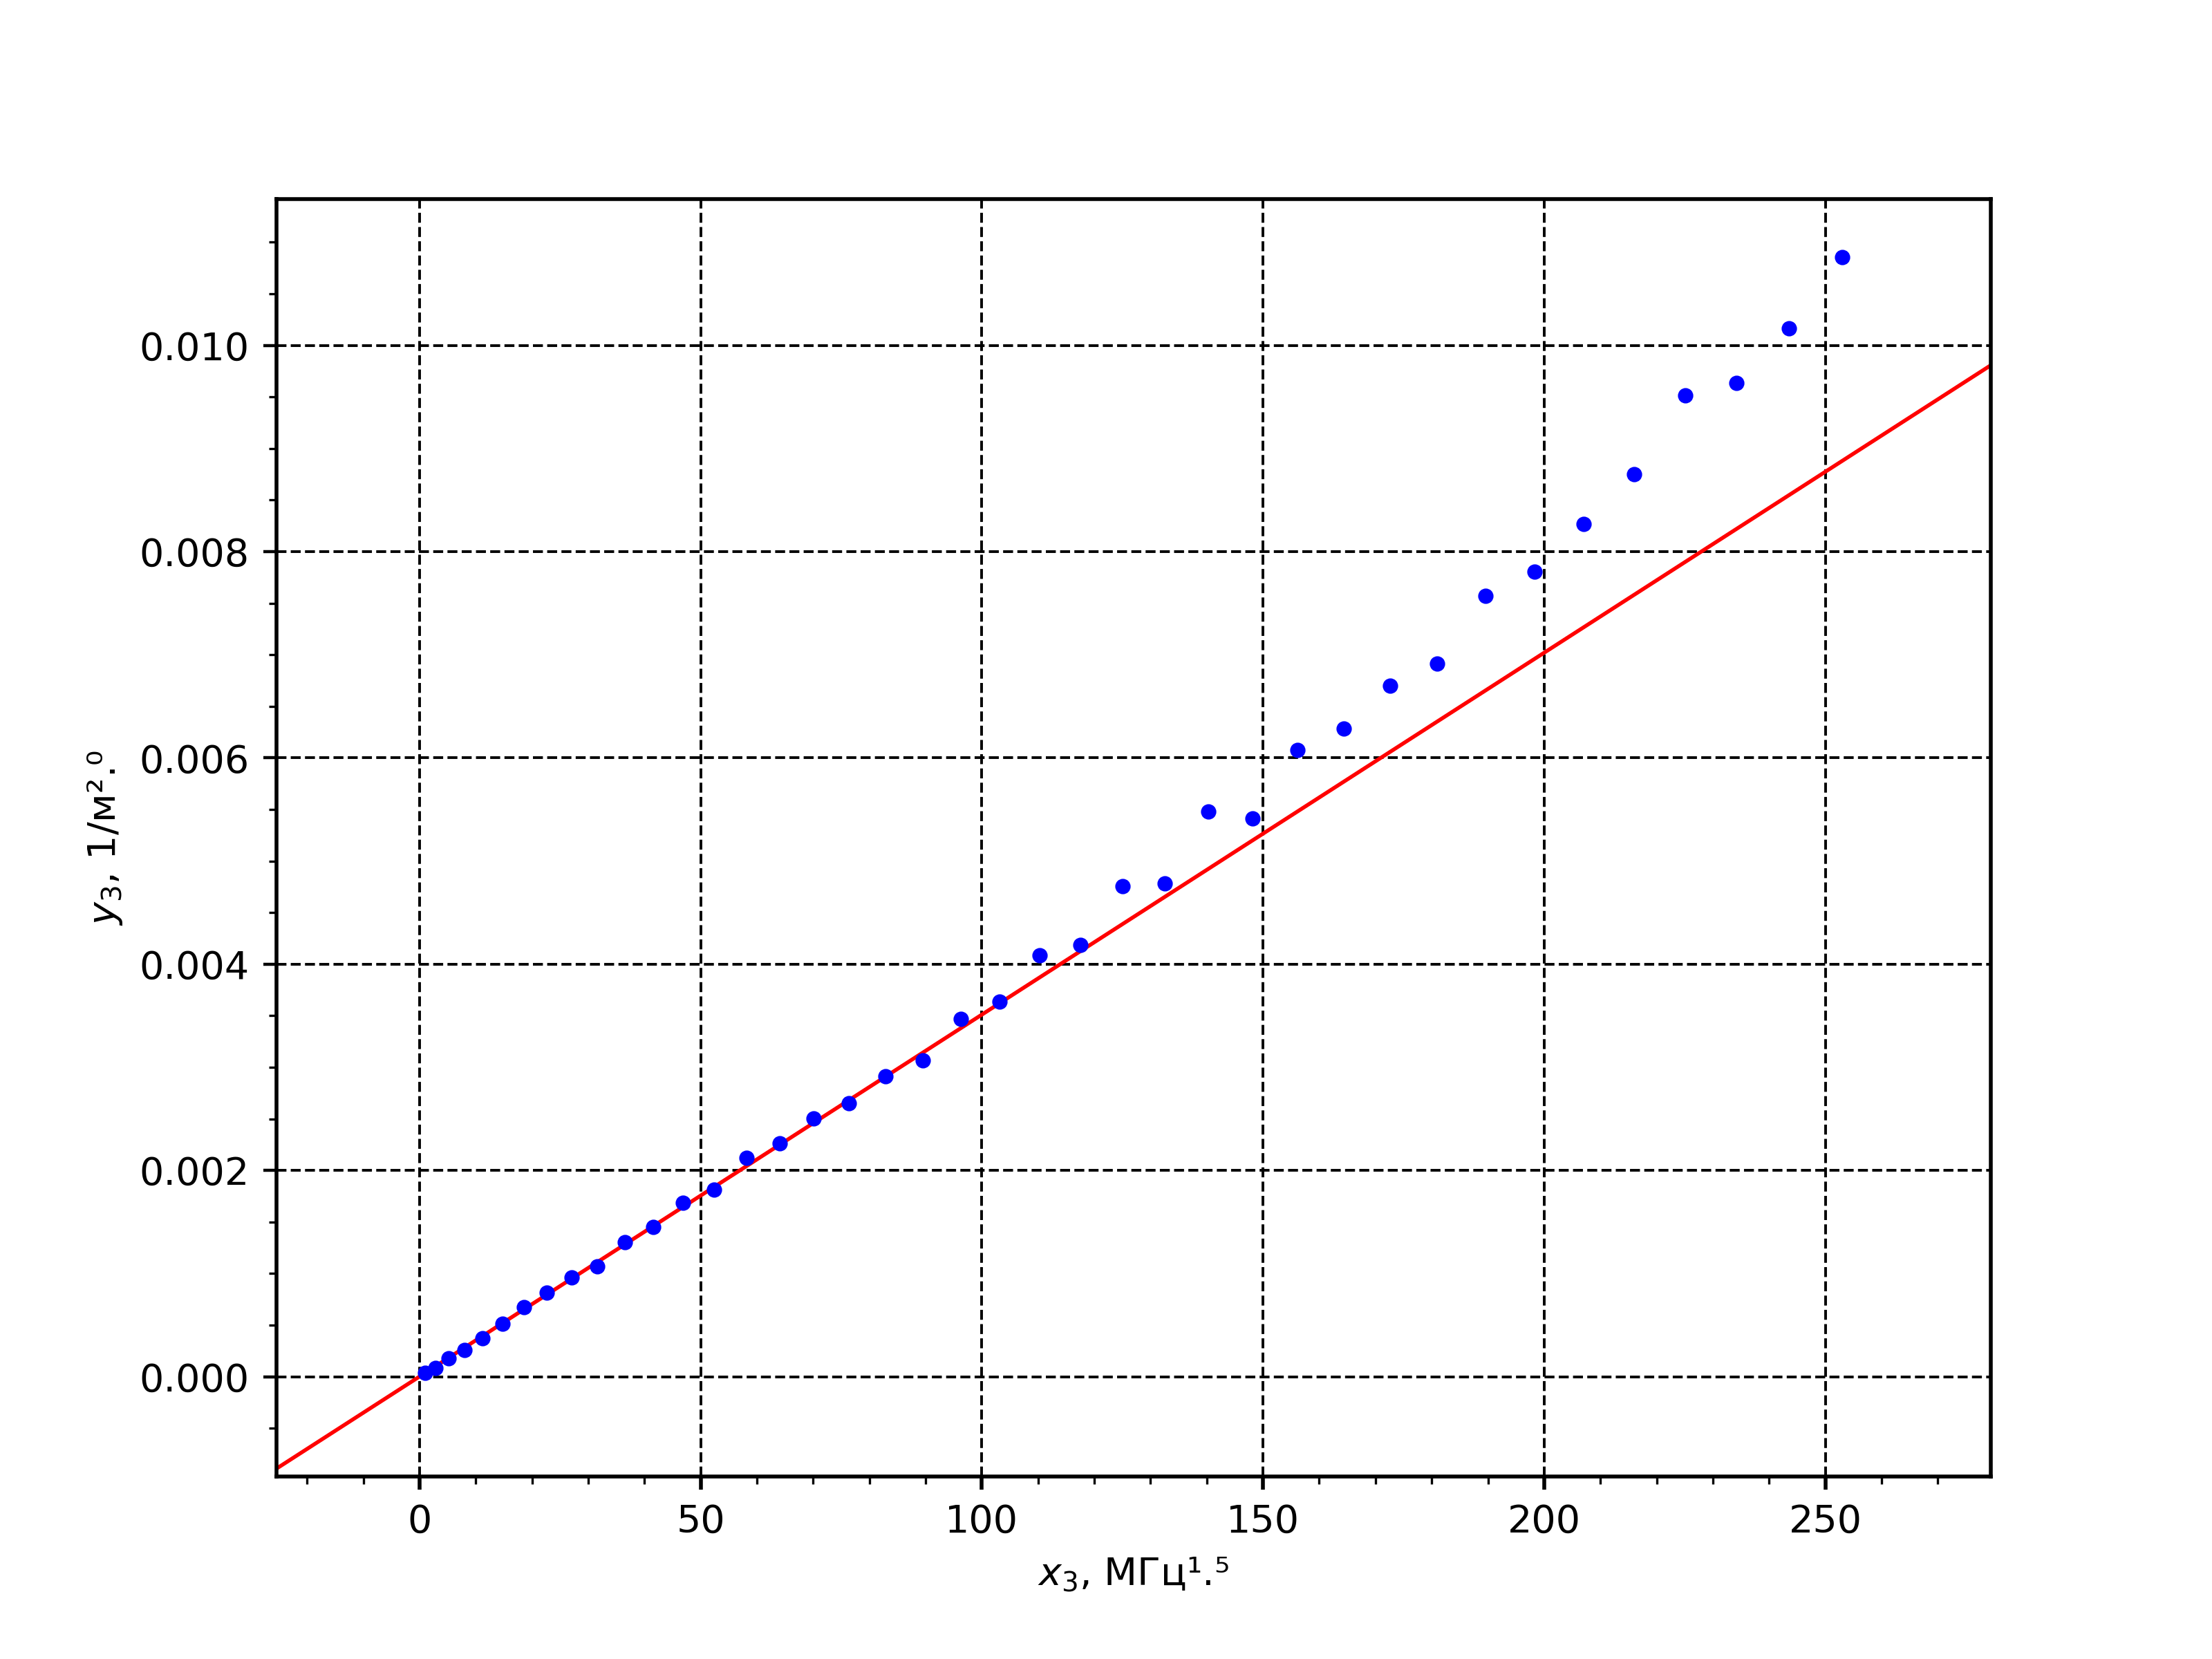
\includegraphics[width=0.8\linewidth]{../img/line3.png}}
\end{figure}
\[
    k_{3} = \left(351 \pm 3\right)\cdot 10^{-7}\;\text{МГц}^{-1.5}\cdot\text{м}^{-2.0}
\]
\[
    \sigma = \left(68{,}7 \pm 1{,}1\right)\cdot 10^{6}\;\text{См} / \text{м}
\]


Фазовая скорость связана с резонансной частотой формулой
\[
    V_{\text{ф}} = \frac{wl}{2 \pi n}
\]

\begin{figure}[ht!]
    \center{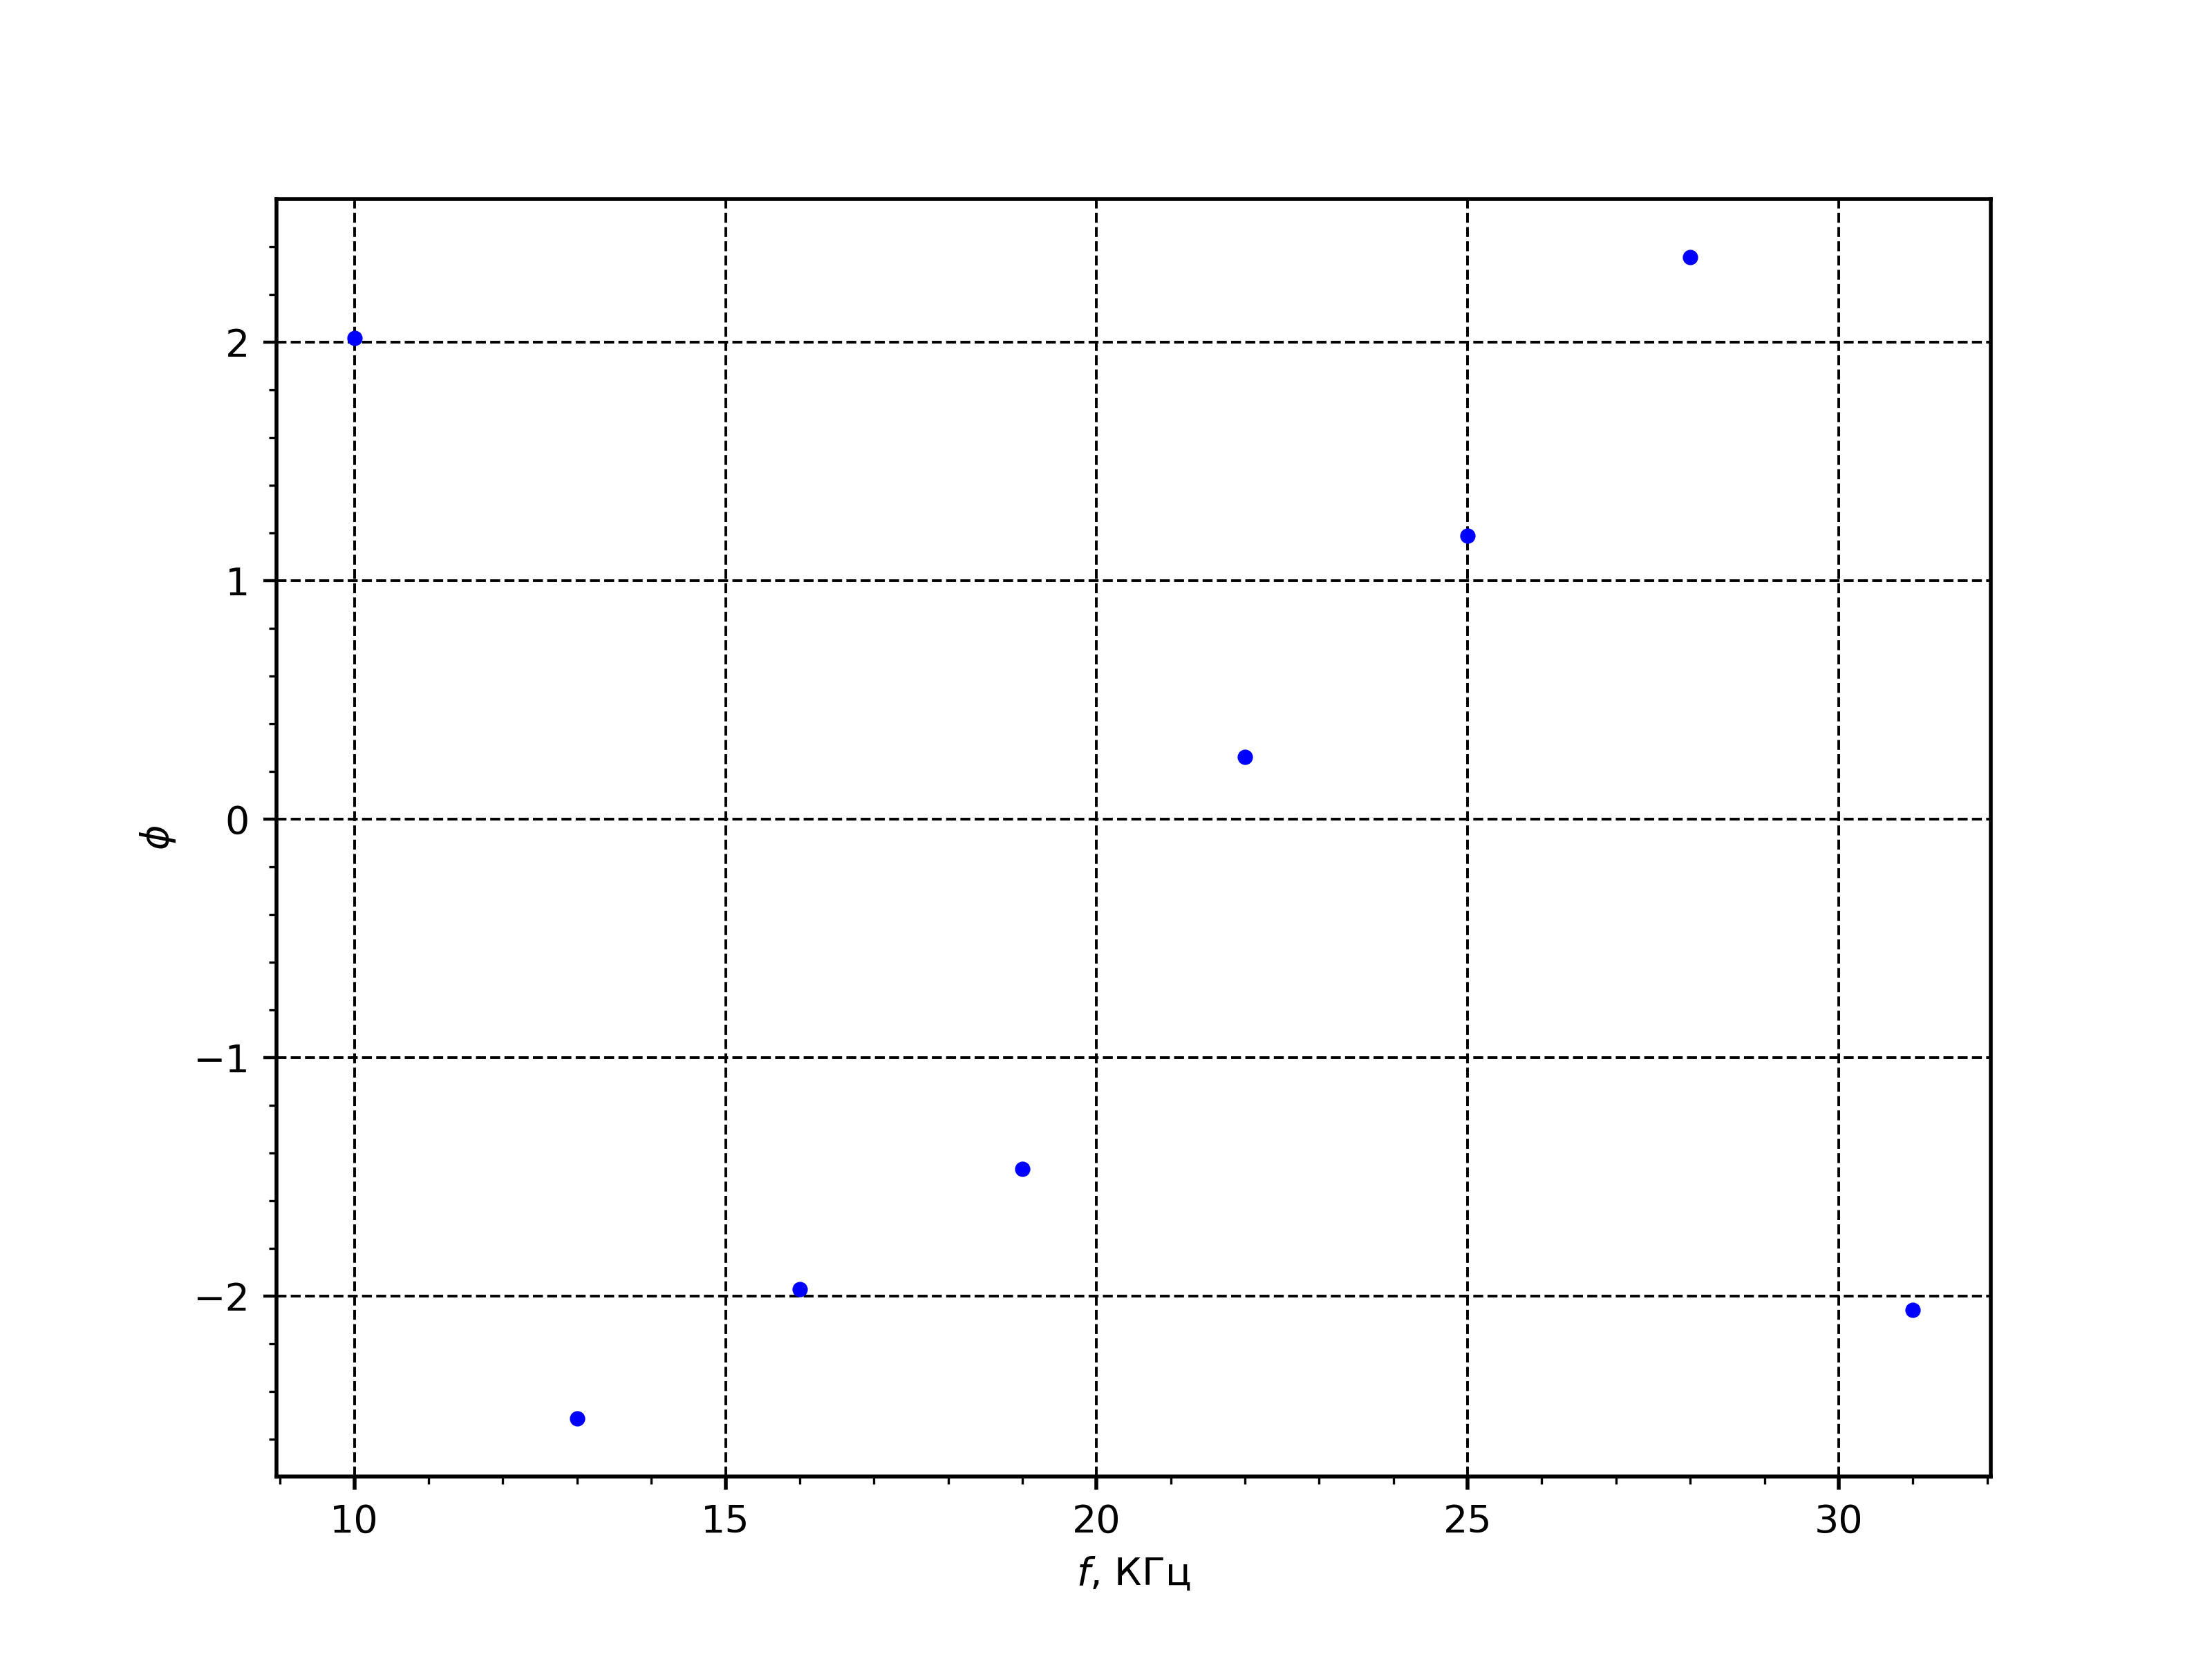
\includegraphics[width=0.8\linewidth]{../img/shit.png}}
\end{figure}
\begin{table}[!ht]
    \centering
    \caption{Измерение фазы от амплитуды}
    \begin{tabular}{|l|l|}
\hline
$f,\;\text{КГц}$ & $\varphi$\\\hline
$10{,}0$ & $2{,}0158552860534504$\\\hline
$13{,}0$ & $-2{,}5132741228718345$\\\hline
$16{,}0$ & $-1{,}9722220547535925$\\\hline
$19{,}0$ & $-1{,}4660765716752369$\\\hline
$22{,}0$ & $0{,}2617993877991494$\\\hline
$25{,}0$ & $1{,}1868238913561442$\\\hline
$28{,}0$ & $2{,}356194490192345$\\\hline
$31{,}0$ & $-2{,}059488517353309$\\\hline
\end{tabular}

\end{table}
График получился линейным (первая и последняя точки лежат на прямой с точностью до $2\pi$), что
соответствует формуле
\[
    k=\frac{\Delta\phi}{l}
\]

\begin{table}[!ht]
    \centering
    \caption{Резонансные частоты}
    \begin{tabular}{|l|l|}
\hline
$f_{R=0},\;\text{КГц}$ & $f_{R\to\infty},\;\text{КГц}$\\\hline
$11{,}2$ & $10{,}7$\\\hline
$21{,}2$ & $20{,}6$\\\hline
$29{,}0$ & $28{,}4$\\\hline
$34{,}6$ & $33{,}8$\\\hline
\end{tabular}

\end{table}

\begin{table}[!ht]
    \centering
    \caption{Распределение напряжений}
    \begin{tabular}{|l|l|l|l|}
\hline
$N$ & $V_{f=10{,}7\;\text{КГц}},\;\text{В}$ & $V_{f=20{,}6\;\text{КГц}},\;\text{В}$ & $V_{f=28{,}4\;\text{КГц}},\;\text{В}$\\\hline
$1{,}0$ & $19{,}0$ & $13{,}0$ & $9{,}0$\\\hline
$2{,}0$ & $10{,}0$ & $6{,}4$ & $12{,}8$\\\hline
$3{,}0$ & $5{,}0$ & $14{,}6$ & $6{,}4$\\\hline
$4{,}0$ & $9{,}4$ & $7{,}0$ & $7{,}6$\\\hline
$5{,}0$ & $17{,}8$ & $11{,}2$ & $7{,}4$\\\hline
$6{,}0$ & $13{,}6$ & $8{,}6$ & $5{,}8$\\\hline
$7{,}0$ & $9{,}6$ & $4{,}4$ & $6{,}2$\\\hline
$8{,}0$ & $6{,}0$ & $9{,}0$ & $4{,}2$\\\hline
$9{,}0$ & $9{,}3$ & $7{,}2$ & $5{,}4$\\\hline
$10{,}0$ & $13{,}8$ & $8{,}6$ & $4{,}6$\\\hline
\end{tabular}

\end{table}
\begin{figure}[ht!]
    \center{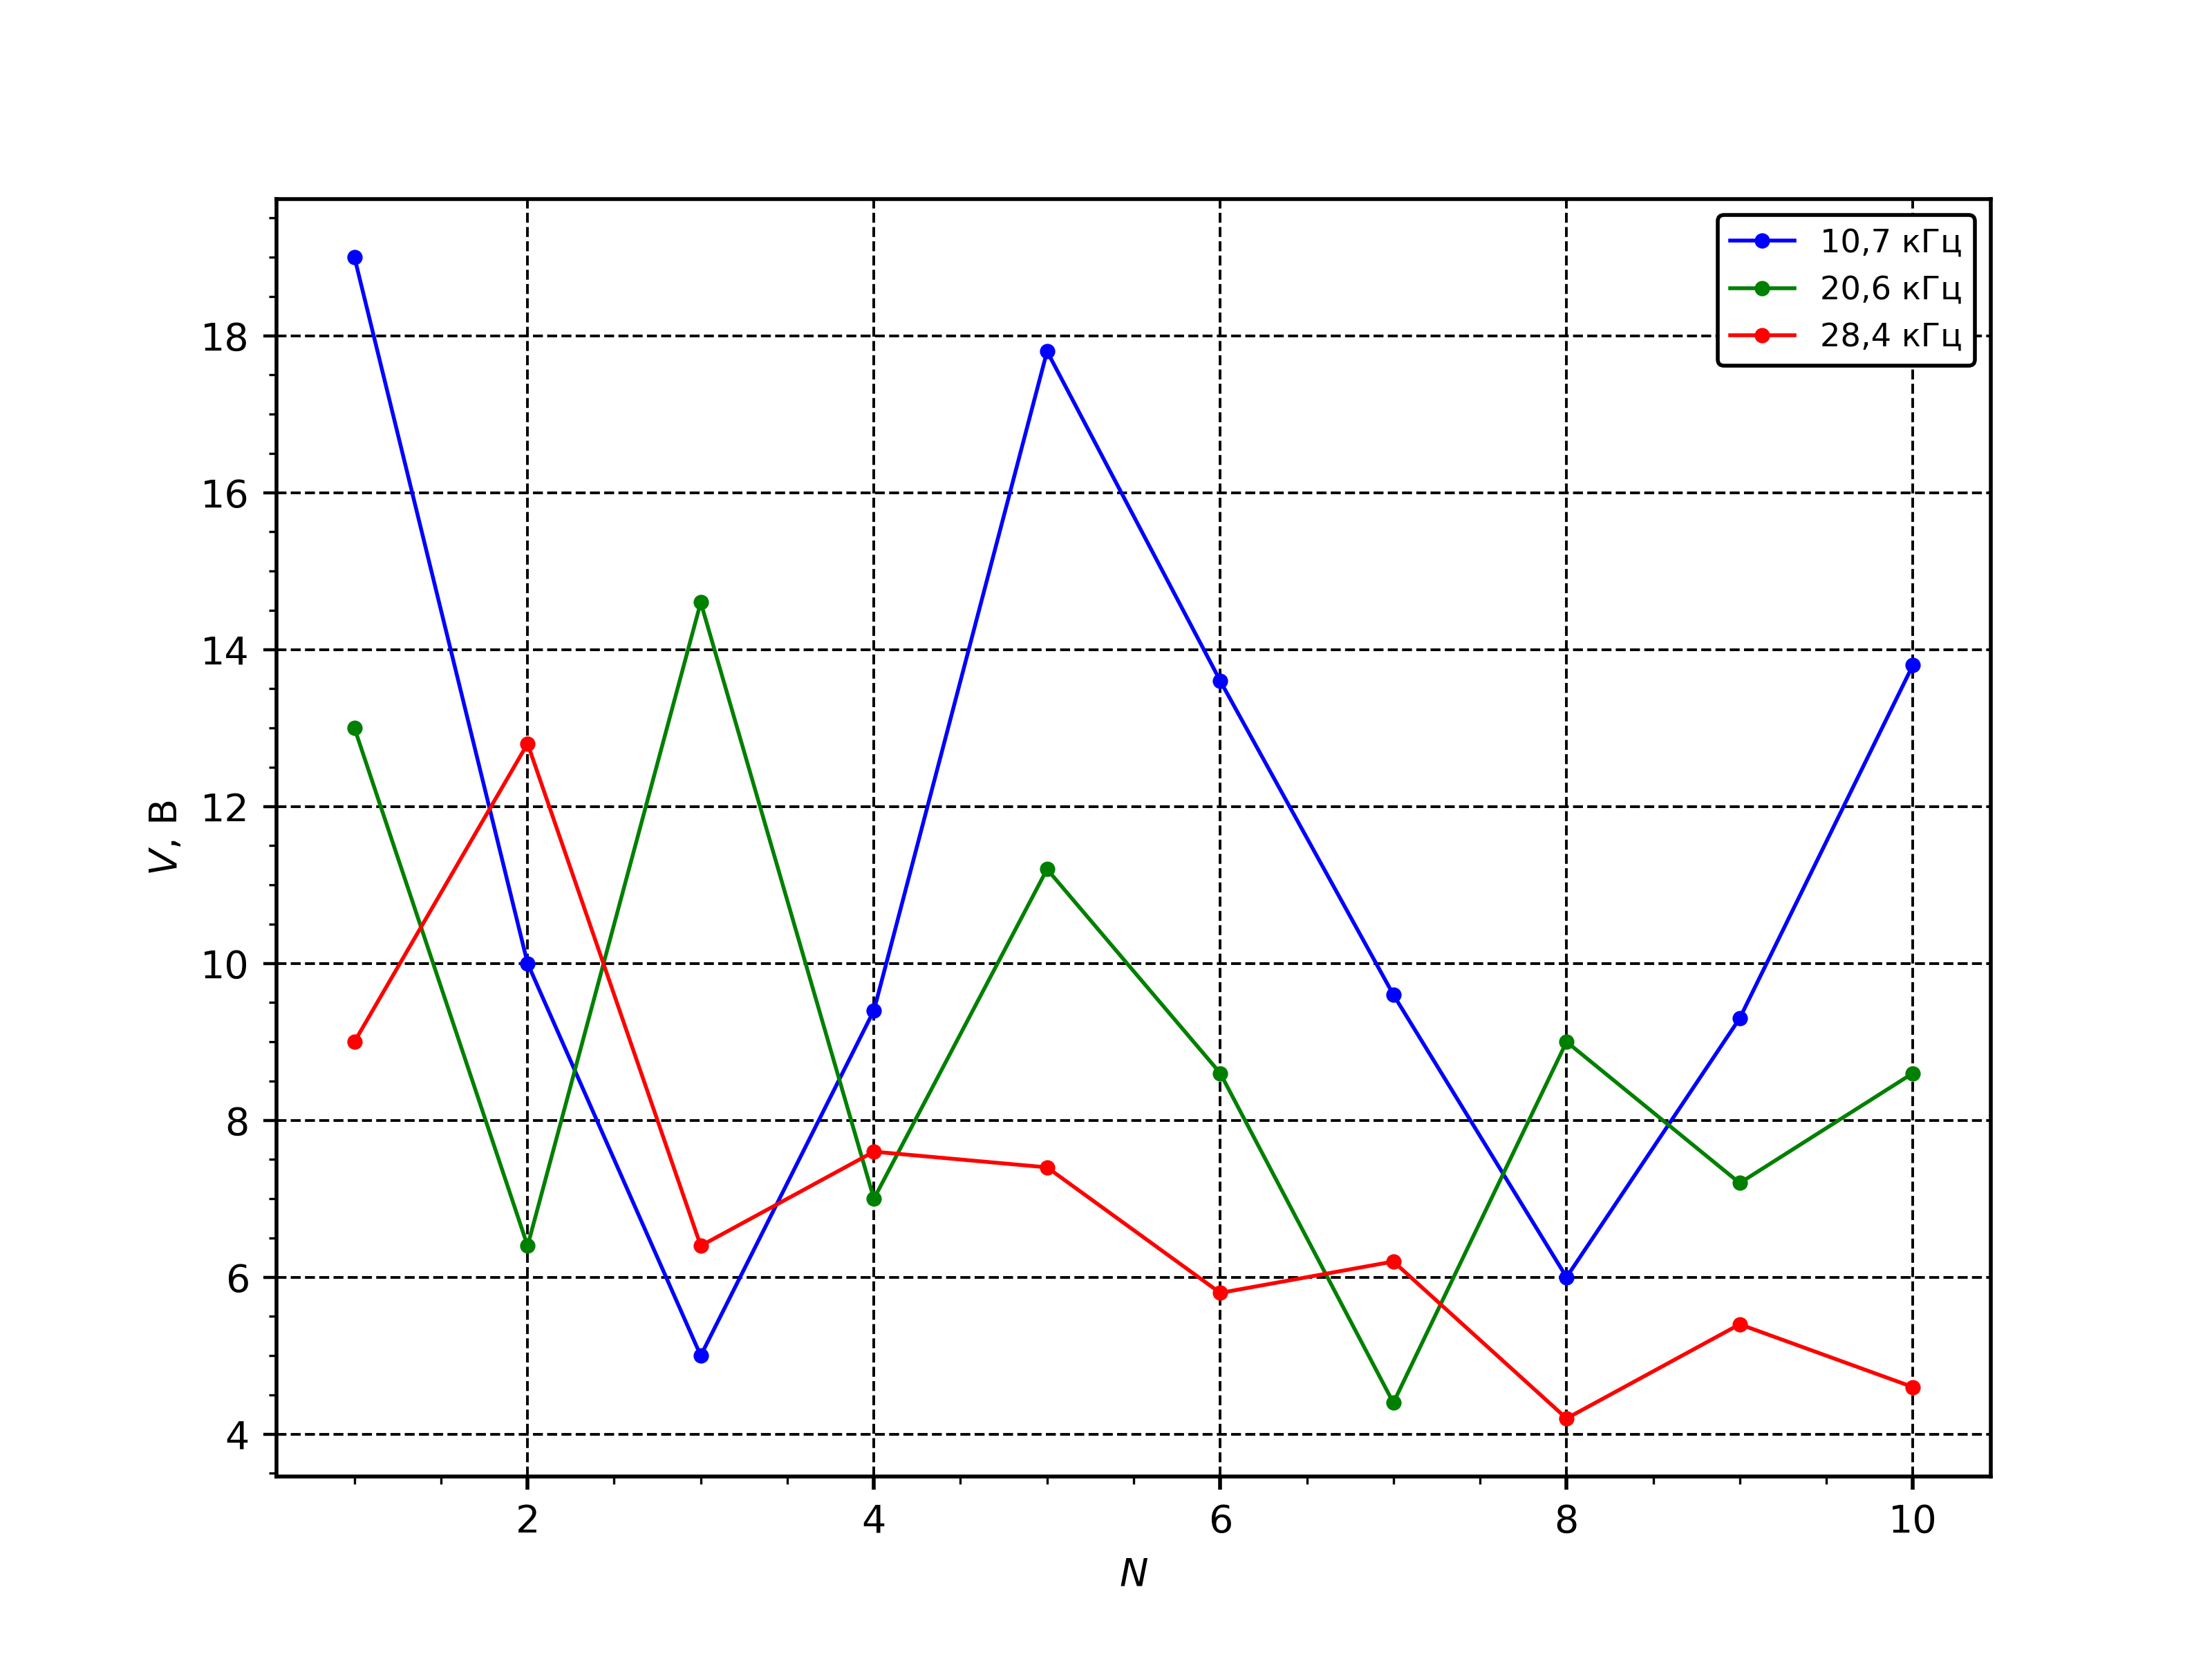
\includegraphics[width=0.8\linewidth]{../img/us.png}}
\end{figure}

